\newpage 
\subsection{Modbus RTU}
\label{subsec:Modbus-RTU}

Der Modbus RTU basiert auf einer Master-Slaves-Architektur. Ein Master kann mittels eines Befehls an den Slave Informationen schicken, worauf der Slave mit einer Antwort den Befehl ausführt, die Informationen verarbeitet und die erfragten Daten an den Master zurückschickt.

%Um den Ablauf des Programm-Codes des installierten Modbus-Systems zu verstehen, wird zunächst die Befehls- und Datenstruktur erklärt. Dann wird ein Überblick über die Abfrage- bzw. Schreibbefehle gegeben. Zum Schluss wird ein Blick auf den Programmablauf geworfen.

\subsubsection*{Datenstruktur und Timing}

Eine Modbus RTU-Nachricht besteht aus mehreren seriell Bytes (8 Bits). Jedem gesendeten Byte geht ein zusätzliches Stop-Bit voraus. Nach dem Byte gibt es mehrere Möglichkeiten, um das gesendete Byte zu beenden. Die meist genutzten Varianten ist zunächst ein Paritätsbit und ein Stopbit oder zwei Stopbits. 
Das Startbit, auch steigende Flanke genannt,  gibt dem Slave das Signal, dass ein Byte kommt. Der Receiver des Slave wird aktiviert. Dann wird das Byte gelesen. Nach dem Byte kommen nun entweder zwei Stopbits oder ein Paritätsbit und ein Stopbit. Beide Arten signalisierten dem Slave-Receiver, dass der Byte zu Ende ist. 

%Wird mit einem Paritätsbit gearbeitet, kann der Slave-Receive kontrollieren, ob die empfangenen acht Bits des Bytes korrekt sind. Es gibt zwei Paritätsarten: \textit{gerade} und \textit{ungerade}. Wird die \textit{gerade} Paritätsart verwendet, so wird das Paritätsbit 1, wenn das Byte eine gerade Anzahl an Einsen hat. Ein Byte bestehend aus "0000 1111" würde das Paritätsbit auf "1" gesetzt; bei "0001 1111" wäre es "0". Die \textit{ungerade} Parität funktioniert nach dem gleichen Prinzip, nur dass das Pariätsbit "1" ist bei einer ungraden Anzahl "1" im gesendeten Byte. Die Hersteller als auch die \textsc{\citeauthor{MODBUS.ORG2002}} empfehlen die Verwendung einer Parität. Mit Startbit, Paritätsbit und Stopbit ist die Bit-Sequenz 11 Bits lang. 

%Wird keine Parität verwendet, so wird anstatt des Paritätsbits ein weiteres Stopbit verwendet, um die Bit-Sequenz wieder 11 Bits lang zu machen. 


Alle Slaves und der Master müssen in einem Netzwerk die gleichen Einstellungen besitzen. Abweichende Einstellungen führen zu Kommunikationsfehlern. Eine weitere wichtige Eigenschaft eines Modbus-System ist die sogenannte \textit{Baudrate}, ihre Einheit ist bps (\textit{bauds per second}). Sie gibt die Geschwindigkeit der Datenübertragung an. Die diskreten Werte für die Geschwindigkeit können zwischen 1200\dots 115200 bps liegen. 


Eine komplette Modbus RTU-Nachricht besteht aus einer Adresse, einer Funktion, Daten und einer \textit{Cyclical Redundancy Checking} (CRC)-Checksumme. Hier steht die Adresse des Slaves im Netzwerk für den der Befehl gilt. Die Adresse darf im Bereich 1\dots 247 liegen.
Danach kommt die Modbus-Funktion. Es können nicht zwei Befehle simultan ausgeführt werden. Für zwei verschiedene Befehle müssen zwei Nachrichten geschickt werden. 
Dann folgen die Datenbytes. Diese bestehen aus mehreren aneinander gereihten Bytes. In einer Nachricht können 0\dots 252 Datenbytes enthalten sein. 
Am Ende jeder Nachricht findet ein CRC-Test statt. Dieser Test kontrolliert die ganze Modbus-Nachricht auf Fehler, unabhängig von den Paritätseinstellungen.
Vor und nach jeder Nachricht gibt es eine von der Baudrate abhängigenes Timeout. Das Timeout verhindert eine zu hohe CPU-Auslastung auf der Masterseite.\citep{MODBUS.ORG2002} \citep{Schleicher2005}


\begin{figure}[htb]
\centering		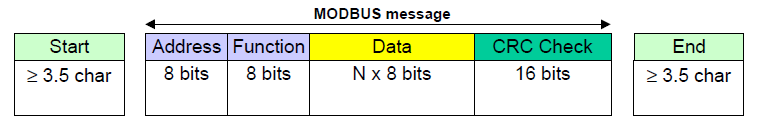
\includegraphics[width=0.90\textwidth]{Pictures/Versuchsaufbau/Modbus_Frame.png}
\caption{Aufbau und Timing einer Modbus RTU-Nachricht \citep{MODBUS.ORG2002}}
\label{fig:}
\end{figure}

\subsubsection*{Befehlsstruktur und Register-Adressen}

Jeder Modbus-Slave hat Informationen oder schreibt Messdaten in seinen internen Speicher. Mögliche Registerspeicher und alle Modbus RTU-Befehle sind im Anhang \ref{Anhang:Modbus} aufgelistet.
Jede Information besitzt eine eindeutige Adresse und hat Lese- bzw. Schreibrechte einprogrammiert.

 Möchte ein Master nun eine Information aus einem Zwischenspeicher lesen oder schreiben bzw. überschreiben, so benötigt er die passende Adresse und für den Zwischenspeicher passenden Befehlstyp.

In der Abbildung \ref{fig:ModbusNachrichtBeispiel} ist beispielhaft eine Druckabfrage eines Drucktransmitters abgebildet. Das Druckwert-Register besteht aus 4 Datenbytes, die zunächst in einen 32 Bit-String und dann in eine REAL-Zahl umgewandelt werden kann. 
Die Anfrage enthält die Startregister-Nummer und die Anzahl der abzufragenden Register. 
Der Slave antwortet auf den Befehl  mit seiner Adresse, den Befehlstyp, die Anzahl der folgenden Datenbytes und mit den Datenbytes selber. Danach erfolgt ein CRC-Test. In grün eingezeichnet sind die Datenbytes und der entsprechende REAL-Zahlenwert. 

\begin{figure}[htb]
\centering		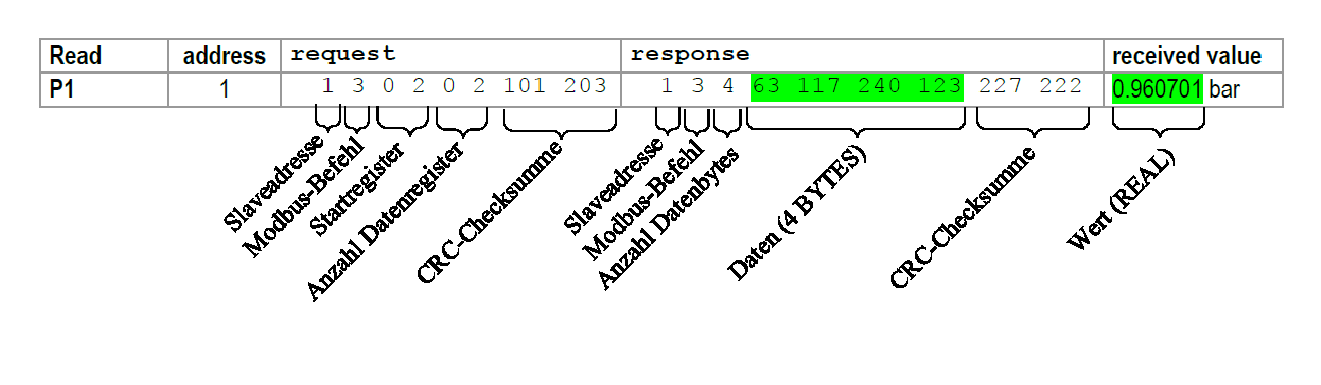
\includegraphics[width=1.0\textwidth]{Pictures/Versuchsaufbau/ModbusBefehlBeispiel.pdf}
\caption{Modbus-Nachrichten Beispiel: Druckabfrage vom Kanal $P1$. Links der Modbusbefehl (\textit{request}) vom Master und rechts die Antwort (\textit{response})}
\label{fig:ModbusNachrichtBeispiel}
\end{figure}


